%! Author = joels
%! Date = 14/06/2021

\section{Multi-Threading Grundlagen}
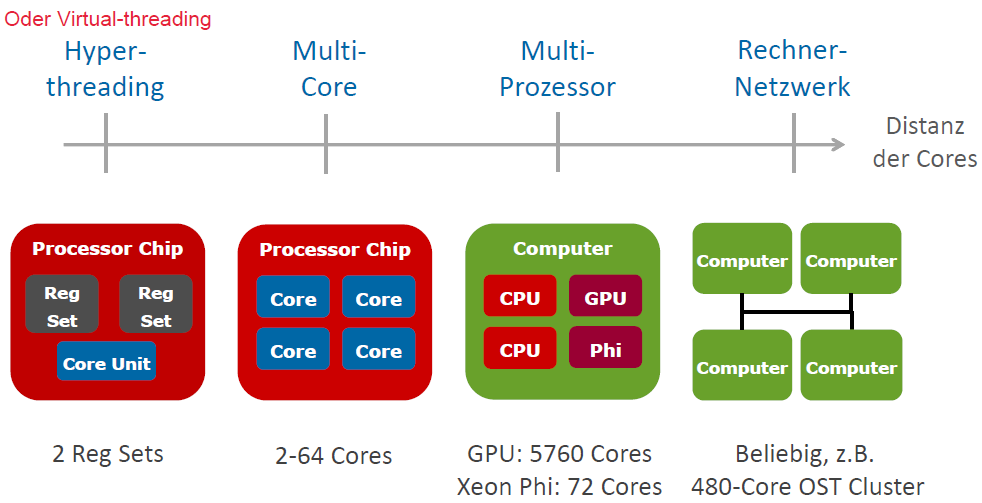
\includegraphics[width=0.97\linewidth]{stufen_parallelisierung}\\
\textcolor{b}{\textbf{Parallelität (Parallelism):}} Mehrere Teilabläufe, welche gleichzeitig auf mehreren Prozessoren/Cores laufen. $\rightarrow$ Schnellere Programme\\
\textcolor{b}{\textbf{Nebenläufigkeit (Concurrency):}} Gleichzeitig oder verzahnt ausführbare Abläufe, welche auf gemeinsame Ressourcen zugreifen (Logisch unabhängig) $\rightarrow$ Einfachere Programme\\
\textcolor{b}{\textbf{User-Level Threads:}} Im Prozess implementiert (keine echte Parallelität)\\
\textcolor{b}{\textbf{Kernel-Level Threads:}} Im Kernel implementiert (Multi-Core Ausnutzung) $\rightarrow$ Kontextwechsel vom Prozess per SW-Interrupt
\subsection{Thread Scheduling}
\textcolor{b}{\textbf{Processor Sharing:}} Mehr Threads als Prozessoren und bei Wartebidingung Proz. an anderen bereiten Thread abgeben.\\
\textcolor{b}{\textbf{Verzahnte Ausführung:}} Prozessor führt Instruktionen von mehreren Threads in Teilsequenzen aus. $\rightarrow$ Quasiparallelität\\
\textcolor{b}{\textbf{Synchron:}} Warten auf Bedingung $\rightarrow$ Waiting Threads\\
\textcolor{b}{\textbf{Asynchron:}} Zeitablauf $\rightarrow$ Nach gewisser Zeit Proz. abgeben\\
\textcolor{b}{\textbf{Kooperativ:}} Threads müssen explizit beim Scheduler in Abständen Kontextwechsel synchron initiieren\\
\textcolor{b}{\textbf{Preemptiv:}} Scheduler kann per Timer-Interrupt den laufenden Thread asynchron unterbrechen
\subsection{Multi Thread Programmierung}
\textbf{JVM ist ein Prozess im Betriebssystem.} $\rightarrow$ Programmierer kann weitere Threads starten\\
Die JVM läuft, solange Threads laufen.\\
\textbf{Ausnahme:} Deamon Threads (z.B. Garbage Collector). Mit \textcolor{b}{System.exit()/Runtime.exit()} kann die JVM direkt terminiert werden (unsauber)
\begin{lstlisting}
// A,B Ausgaben können durcheinander sein:
public class MultiThreadTest {
    public static void main (String[] args ) {
        var a = new Thread(Thread(() -> multiPrint("A"));
        var b = new Thread(Thread(() -> multiPrint("B"));
        a.start(); b.start();
        System.out.println("main finished");
    }
    static void multiPrint (String label) {
        for (int i = 0; i < 10; i++) {
            System.out.println(label + ": " + i);
        } } }
// Explizite Runnable-Implementation:
class SimpleLogic implements Runnable {
    @Override
    public void run () {
        // thread behavior
    } }
var myThread = new Thread(new SimpleLogic());
myThread.start();
// Sub-Klasse von Thread
class SimpleThread extends Thread {
    @Override
    public void run ()
        // thread behavior
    } }
var myThread = new SimpleThread(); myThread.start();
\end{lstlisting}
\begin{minipage}{0.4\linewidth}
    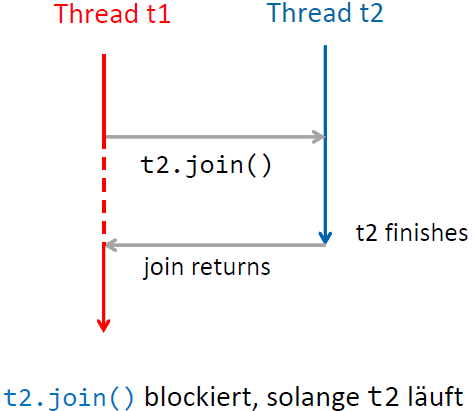
\includegraphics{thread_join}
\end{minipage}
\begin{minipage}{0.5\linewidth}
    \textcolor{red}{t1} wartet, bis \textcolor{b}{t2} fertig ist.\\
    \textbf{Warten:}\\
    Thread.sleep(milliseconds)\\
    \textbf{Prozessor freigeben:}\\
    Thread.yield()\\
    \textbf{Von aussen Unterbrechen:}\\
    myThread.interrupt()\\
    \textbf{Aktuelle Thread-Instanz:}\\
    Thread currentThread()\\
    \textbf{Als Deamon markieren:}\\
    void setDeamon(boolean on)
\end{minipage}